%=============================================================================
%  Rapport ICA — Algorithmes Classiques et Stochastiques
%  M2 Data Science — Réduction de dimension — Avril 2026
%
%  Compilation : pdflatex rapport_ICA.tex  (2 passes pour les références)
%
%  Figures attendues dans le dossier figures/ :
%    fig_sources.png        — sources vraies + mélanges (section 1)
%    fig_infomax.png        — sources estimées Infomax + convergence (section 2)
%    fig_fastica.png        — sources estimées FastICA (section 3)
%    fig_sgd.png            — sources estimées SGD-ICA + courbe lr (section 4)
%    fig_adam.png           — sources estimées Adam-ICA (section 5)
%    fig_benchmark.png      — barplot Amari Index (section 6)
%    fig_convergence.png    — courbes de convergence toutes méthodes (section 6)
%    fig_scalability.png    — temps d'exécution vs n_samples (section 7)
%    fig_vae_beta.png       — effet de beta sur z (section 8)
%    fig_vae_lambda.png     — effet de lambda_HSIC sur corrélation (section 8)
%    fig_vae_sources.png    — sources VAE-ICA vs vraies (section 8)
%    fig_eeg_fastica.png    — composantes FastICA sur EEG (section 9)
%    fig_eeg_corr.png       — matrices de corrélation EEG (section 9)
%=============================================================================

\documentclass[12pt, a4paper]{article}

%── Encodage & langue ──────────────────────────────────────────────────────────
\usepackage[utf8]{inputenc}
\usepackage[T1]{fontenc}
\usepackage[french]{babel}
\usepackage{csquotes}

%── Mise en page ──────────────────────────────────────────────────────────────
\usepackage[top=2.5cm, bottom=2.5cm, left=2.5cm, right=2.5cm]{geometry}
\usepackage{setspace}
\onehalfspacing
\usepackage{parskip}
\setlength{\parindent}{0pt}

%── Typographie ───────────────────────────────────────────────────────────────
\usepackage{lmodern}
\usepackage{microtype}
\usepackage{xcolor}
\definecolor{accent}{HTML}{2c3e50}
\definecolor{blue}{HTML}{3498db}
\definecolor{red}{HTML}{e74c3c}
\definecolor{green}{HTML}{27ae60}
\definecolor{purple}{HTML}{9b59b6}
\definecolor{orange}{HTML}{f39c12}
\definecolor{codebg}{HTML}{f8f9fa}
\definecolor{codefg}{HTML}{c0392b}

%── Maths ─────────────────────────────────────────────────────────────────────
\usepackage{amsmath, amssymb, amsthm, bm}
\usepackage{mathtools}

%── Figures & tableaux ────────────────────────────────────────────────────────
\usepackage{graphicx}
\usepackage{float}
\usepackage{caption}
\usepackage{subcaption}
\usepackage{booktabs}
\usepackage{array}
\usepackage{multirow}
\captionsetup{font=small, labelfont=bf, labelsep=period}
\graphicspath{{figures/}}

%── Code ──────────────────────────────────────────────────────────────────────
\usepackage{listings}
\lstset{
  backgroundcolor=\color{codebg},
  basicstyle=\ttfamily\small,
  keywordstyle=\color{blue}\bfseries,
  stringstyle=\color{green},
  commentstyle=\color{gray}\itshape,
  frame=single, framerule=0pt,
  rulecolor=\color{gray!30},
  numbers=left, numberstyle=\tiny\color{gray},
  breaklines=true, breakatwhitespace=true,
  language=Python,
  showstringspaces=false,
  xleftmargin=1em, xrightmargin=0.5em,
}

%── Boîtes colorées ───────────────────────────────────────────────────────────
\usepackage{tcolorbox}
\tcbuselibrary{skins, breakable}

\newtcolorbox{definitionbox}[1]{
  colback=blue!6, colframe=blue!60!black,
  title=#1, fonttitle=\bfseries,
  breakable, arc=3pt
}
\newtcolorbox{formulabox}{
  colback=red!5, colframe=red!60!black,
  breakable, arc=3pt
}
\newtcolorbox{notebox}{
  colback=orange!8, colframe=orange!70!black,
  breakable, arc=3pt
}

%── Hyperliens ────────────────────────────────────────────────────────────────
\usepackage[colorlinks=true, linkcolor=accent, citecolor=blue, urlcolor=blue]{hyperref}

%── En-tête / pied de page ────────────────────────────────────────────────────
\usepackage{fancyhdr}
\pagestyle{fancy}
\fancyhf{}
\fancyhead[L]{\small\color{gray} ICA — Algorithmes Classiques \& Stochastiques}
\fancyhead[R]{\small\color{gray} M2 Data Science — 2026}
\fancyfoot[C]{\small\thepage}
\renewcommand{\headrulewidth}{0.4pt}

%── Macros ────────────────────────────────────────────────────────────────────
\newcommand{\V}{\mathbf{V}}        % matrice de séparation
\newcommand{\W}{\mathbf{W}}        % matrice de mélange A
\newcommand{\x}{\mathbf{x}}        % observation
\newcommand{\s}{\mathbf{s}}        % sources
\newcommand{\y}{\mathbf{y}}        % sources estimées
\newcommand{\E}{\mathbb{E}}        % espérance
\newcommand{\R}{\mathbb{R}}
\newcommand{\norm}[1]{\left\|#1\right\|}
\newcommand{\algo}[1]{\textcolor{accent}{\textbf{#1}}}

%=============================================================================
\begin{document}
%=============================================================================

%── Page de titre ─────────────────────────────────────────────────────────────
\begin{titlepage}
  \centering
  \vspace*{2cm}
  {\color{accent}\rule{\linewidth}{1.5pt}}\\[0.8em]
  {\Huge\bfseries\color{accent}
    Analyse en Composantes Indépendantes\\[0.4em]
    \large Algorithmes Classiques et Stochastiques
  }\\[0.6em]
  {\color{accent}\rule{\linewidth}{1.5pt}}\\[2cm]

  \begin{tcolorbox}[colback=accent!5, colframe=accent, arc=5pt,
                    width=0.85\linewidth]
    \centering
    \textbf{Algorithmes implémentés}\\[0.5em]
    \begin{tabular}{ll}
      \textcolor{red}{$\blacktriangleright$} & Infomax ICA — gradient batch (Bell \& Sejnowski, 1995) \\
      \textcolor{purple}{$\blacktriangleright$} & FastICA — point fixe (Hyvärinen, 1999) \\
      \textcolor{blue}{$\blacktriangleright$} & SGD-ICA — gradient stochastique \\
      \textcolor{green}{$\blacktriangleright$} & Adam-ICA — optimiseur adaptatif \\
      \textcolor{orange}{$\blacktriangleright$} & VAE-ICA — autoencodeur variationnel + HSIC \\
    \end{tabular}
  \end{tcolorbox}

  \vfill
  {\large Master 2 Data Science\\[0.3em]
   Réduction de dimension\\[0.3em]
   \textbf{Avril 2026}}
\end{titlepage}

%── Table des matières ────────────────────────────────────────────────────────
\tableofcontents
\newpage

%=============================================================================
\section{Introduction et contexte}
%=============================================================================

\begin{definitionbox}{Séparation aveugle de sources (BSS)}
L'Analyse en Composantes Indépendantes (ICA) est une méthode de \textbf{séparation aveugle de
sources}. Étant donné un vecteur d'observations $\x \in \R^d$, on suppose qu'il résulte d'un
mélange linéaire de $k$ sources statistiquement indépendantes $\s \in \R^k$ :
\begin{equation}
  \x = \W \s, \qquad \W \in \R^{d \times k}
\end{equation}
L'objectif est d'estimer la \textbf{matrice de séparation} $\V \in \R^{k \times d}$ telle que
\begin{equation}
  \hat{\s} = \V \x \approx \s
\end{equation}
à une permutation et mise à l'échelle des composantes près.
\end{definitionbox}

\subsection{Prétraitement : centrage et blanchiment}

Avant toute estimation, les données sont prétraitées :
\begin{enumerate}
  \item \textbf{Centrage} : $\x \leftarrow \x - \bar{\x}$.
  \item \textbf{Blanchiment PCA} : on calcule la décomposition en valeurs propres de la matrice de
        covariance $\Sigma = \E[\x\x^\top]$, et on transforme les données de sorte que
        $\E[\x_{\text{blanc}}\x_{\text{blanc}}^\top] = I_k$.
        Cela réduit aussi la dimension de $d$ à $k$ si $k < d$.
\end{enumerate}
La matrice de séparation cherchée opère sur les données blanchies :
\[
  \hat{\s} = \V \underbrace{W_{\text{pca}}(\x - \bar{\x})}_{\x_{\text{blanc}}}
\]

\subsection{Mesure de performance : indice d'Amari}

L'indice d'Amari mesure l'écart entre la matrice de séparation estimée et la vraie matrice de
mélange, en étant invariant aux permutations et aux changements d'échelle des composantes
\cite{amari1996}. Un indice proche de 0 indique une séparation quasi-parfaite.

\begin{formulabox}
\[
  \text{Amari}(\hat{\V}, \W) =
  \frac{1}{2k} \sum_{i=1}^{k}
  \left( \frac{\sum_j |p_{ij}|}{\max_j |p_{ij}|} - 1 \right)
  + \frac{1}{2k} \sum_{j=1}^{k}
  \left( \frac{\sum_i |p_{ij}|}{\max_i |p_{ij}|} - 1 \right)
\]
où $P = \hat{\V} \W$ est la matrice produit globale.
\end{formulabox}

%=============================================================================
\section{Données synthétiques}
%=============================================================================

On simule un problème BSS classique avec $n = 3000$ échantillons et $k = 3$ sources de natures
différentes :

\begin{itemize}
  \item \textbf{Laplace} : super-gaussienne ($\kappa > 0$), à queues lourdes — typique des signaux
        audio ou EEG.
  \item \textbf{Sinusoïde} : sous-gaussienne ($\kappa < 0$), distribution uniforme sur un arc de
        cercle.
  \item \textbf{Uniforme} : sous-gaussienne ($\kappa < 0$), distribution plate sur $[-1, 1]$.
\end{itemize}

La matrice de mélange $\W \in \R^{3 \times 3}$ est générée aléatoirement (colonnes normalisées).

\begin{lstlisting}[caption={Génération des données synthétiques}]
from experiments.benchmark import make_sources

S, A, X = make_sources(
    n_samples=3000,
    n_sources=3,
    source_type='mixed',   # Laplace + sinusoide + uniforme
    random_state=42
)
# S : (3000, 3)  sources independantes vraies
# A : (3, 3)     matrice de melange
# X : (3000, 3)  melanges observes
\end{lstlisting}

\begin{figure}[H]
  \centering
  \includegraphics[width=\linewidth]{fig_sources.png}
  \caption{Sources indépendantes $s_1, s_2, s_3$ (colonne gauche) et mélanges observés
           $x_1, x_2, x_3$ (colonne droite). Chaque mélange combine les trois sources
           via la matrice $\mathbf{A}$.}
  \label{fig:sources}
\end{figure}

%=============================================================================
\section{Algorithmes classiques}
%=============================================================================

%─────────────────────────────────────────────────────────────────────────────
\subsection{Infomax ICA — gradient batch (Bell \& Sejnowski, 1995)}
%─────────────────────────────────────────────────────────────────────────────

\textbf{Principe.}
Infomax \cite{bell1995} maximise l'entropie de la sortie $\y = g(\V\x)$, ce qui revient à
maximiser la log-vraisemblance du modèle ICA sous une densité source choisie.
Le \textbf{gradient naturel} (Amari, 1998) précondionne la mise à jour par la métrique de
Fisher, la rendant invariante à l'échelle de $\V$ :

\begin{formulabox}
\[
  \V \;\leftarrow\; \V + \eta \left( I - \frac{1}{n}\tanh(\y)\y^\top \right) \V,
  \qquad \y = \V\,\x_{\text{blanc}}
\]
\end{formulabox}

La non-linéarité $\tanh$ correspond à une densité source Laplacienne (super-gaussienne).
L'algorithme traite l'intégralité du dataset à chaque itération, ce qui le rend exact
mais non scalable pour $n \gg 10^4$.

%─────────────────────────────────────────────────────────────────────────────
\subsection{FastICA — algorithme point fixe (Hyvärinen, 1999)}
%─────────────────────────────────────────────────────────────────────────────

\textbf{Principe.}
FastICA \cite{hyvarinen1999} maximise la néguentropie $J(y) \approx [\E\{G(y)\} - \E\{G(\nu)\}]^2$
via un algorithme de point fixe à convergence quadratique (Newton-like).
Les composantes sont extraites une par une (\textit{déflation de Gram-Schmidt}) :

\begin{formulabox}
\[
  \mathbf{w} \;\leftarrow\; \E\{\x\,g(\mathbf{w}^\top\x)\} - \E\{g'(\mathbf{w}^\top\x)\}\,\mathbf{w},
  \qquad \mathbf{w} \;\leftarrow\; \mathbf{w}/\|\mathbf{w}\|
\]
\end{formulabox}

\textbf{Fonctions de contraste $G$ et $g = G'$ :}

\begin{center}
\begin{tabular}{lll}
\toprule
\textbf{Option} & $G(u)$ & $g(u)$ \\
\midrule
\texttt{logcosh} (défaut) & $\log\cosh u$ & $\tanh u$ \\
\texttt{exp}              & $-e^{-u^2/2}$ & $u\,e^{-u^2/2}$ \\
\texttt{cube}             & $u^4/4$       & $u^3$ \\
\bottomrule
\end{tabular}
\end{center}

Sans paramètre de pas à régler, FastICA converge en général en moins de 100 itérations
et offre les meilleures performances sur des datasets de taille modérée.

%=============================================================================
\section{Algorithmes stochastiques}
%=============================================================================

%─────────────────────────────────────────────────────────────────────────────
\subsection{SGD-ICA — gradient stochastique sur le critère Infomax}
%─────────────────────────────────────────────────────────────────────────────

\textbf{Principe.}
SGD-ICA applique la règle du gradient naturel Infomax sur des \textbf{mini-batches}
$\mathcal{B} \subset \{1,\ldots,n\}$ de taille $m \ll n$, tirés aléatoirement à chaque étape :

\begin{formulabox}
\[
  \V \;\leftarrow\; \V + \eta_t \left( I - \frac{1}{m}\tanh(\y_\mathcal{B})\y_\mathcal{B}^\top
  \right) \V, \qquad \y_\mathcal{B} = \V X_\mathcal{B}
\]
\end{formulabox}

Trois planifications du taux d'apprentissage sont disponibles :
\texttt{constant}, \texttt{inv\_sqrt} ($\eta_t = \eta_0/\sqrt{t}$),
et \texttt{cosine} ($\eta_t = \frac{\eta_0}{2}(1+\cos(\pi t/T))$).
L'empreinte mémoire est constante en $m$, ce qui rend l'algorithme compatible avec
des datasets ne tenant pas en RAM et avec le traitement en flux.

%─────────────────────────────────────────────────────────────────────────────
\subsection{Adam-ICA — optimiseur adaptatif}
%─────────────────────────────────────────────────────────────────────────────

\textbf{Principe.}
Adam \cite{kingma2015} maintient des estimateurs du premier ($m_t$, direction) et du second
($v_t$, variance) moment du gradient naturel, adaptant le pas \emph{par paramètre} :

\begin{formulabox}
\[
  m_t = \beta_1 m_{t-1} + (1{-}\beta_1)\,G_t, \quad
  v_t = \beta_2 v_{t-1} + (1{-}\beta_2)\,G_t^2
\]
\[
  \V \;\leftarrow\; \V + \eta\,\frac{\hat{m}_t}{\sqrt{\hat{v}_t}+\varepsilon},
  \qquad \hat{m}_t = \tfrac{m_t}{1-\beta_1^t},\;\; \hat{v}_t = \tfrac{v_t}{1-\beta_2^t}
\]
\end{formulabox}

Hyperparamètres standards : $\beta_1 = 0.9$, $\beta_2 = 0.999$, $\varepsilon = 10^{-8}$.
Par rapport à SGD-ICA, Adam converge en 2 à 3 fois moins d'epochs grâce à l'adaptation
automatique du pas, au prix d'un surcoût mémoire de deux matrices de moments ($O(3kd)$
contre $O(kd)$).

%=============================================================================
\section{Benchmark et visualisations}
%=============================================================================

Le benchmark compare les quatre algorithmes sur le dataset synthétique ($n=3000$, $k=3$,
sources mixtes, \texttt{random\_state=42}) via l'indice d'Amari (invariant à la permutation
et à l'échelle des composantes).

\begin{figure}[H]
  \centering
  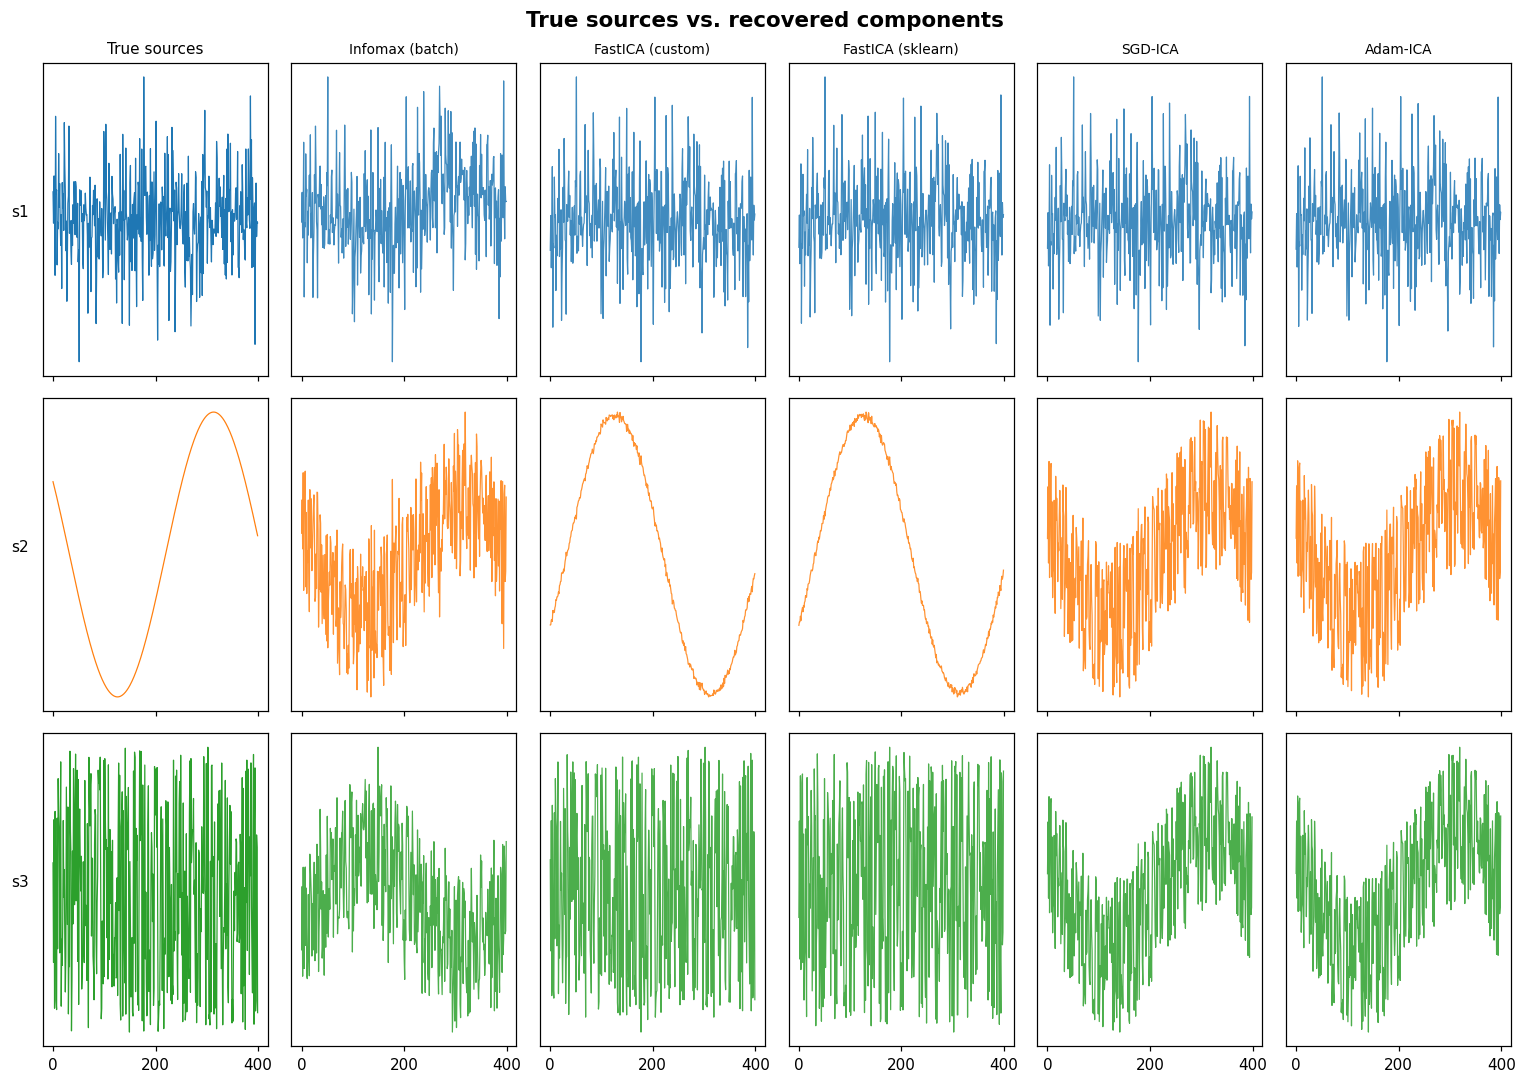
\includegraphics[width=\linewidth]{images/plot2.png}
  \caption{Sources vraies vs sources estimées par chaque algorithme (Infomax, FastICA,
           SGD-ICA, Adam-ICA). Les corrélations croisées $|r|$ quantifient la qualité de
           séparation composante par composante.}
  \label{fig:sources_est}
\end{figure}

\begin{figure}[H]
  \centering
  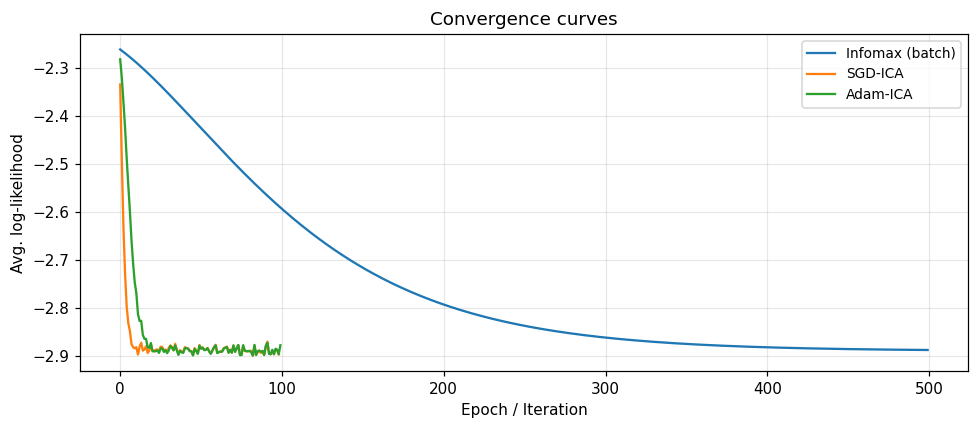
\includegraphics[width=\linewidth]{images/plot3.png}
  \caption{Gauche : indice d'Amari par algorithme (barres, $\downarrow$ meilleur).
           Droite : courbes de convergence (log-vraisemblance ou perte) au fil des
           itérations/epochs.}
  \label{fig:benchmark}
\end{figure}

%=============================================================================
\section{Scalabilité}
%=============================================================================

Les méthodes stochastiques (SGD-ICA, Adam-ICA) opèrent sur des mini-batches de taille fixe
$m$, ce qui maintient un coût mémoire constant quel que soit $n$. On mesure le temps
d'entraînement (20~epochs) pour $n \in \{1\,000,\,5\,000,\,10\,000,\,30\,000\}$ :

\begin{figure}[H]
  \centering
  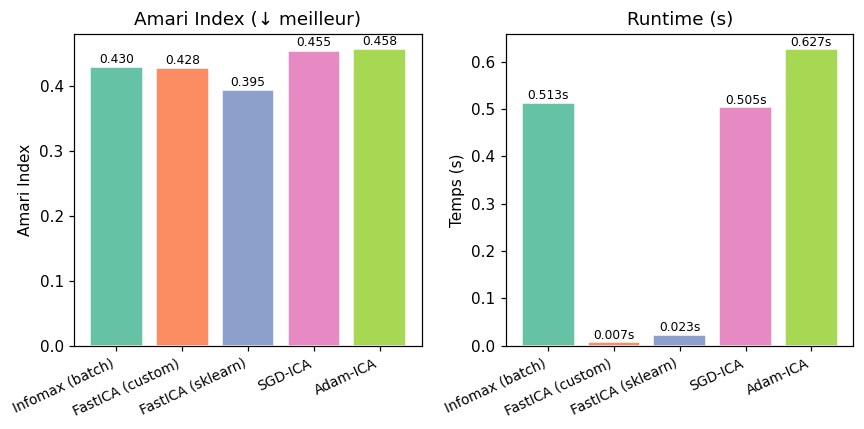
\includegraphics[width=0.80\linewidth]{images/plot4.png}
  \caption{Temps d'entraînement en fonction du nombre d'échantillons. Infomax batch croît
           linéairement avec $n$ et devient prohibitif pour $n > 10^4$, tandis que
           SGD-ICA et Adam-ICA restent quasi-constants (mini-batch de taille fixe $m=128$).}
  \label{fig:scalability}
\end{figure}

%=============================================================================
\section{VAE-ICA — Autoencodeur variationnel}
%=============================================================================

\subsection{Motivation}

Les algorithmes ICA classiques supposent une forme paramétrique fixe pour la densité des
sources ($\tanh \sim$ Laplace, $u^3 \sim$ sous-gaussien). \textbf{VAE-ICA} apprend
directement la distribution des sources et impose l'indépendance dans l'espace latent via
un critère non-paramétrique (HSIC), sans hypothèse sur $p_j$.

\subsection{Architecture et fonction de perte}

\begin{center}
\begin{tabular}{lll}
\toprule
\textbf{Module} & \textbf{E/S} & \textbf{Description} \\
\midrule
Encodeur        & $\x \to \bm{\mu}, \bm{\sigma} \in \R^k$ & MLP : Linear $\to$ ReLU $\to$ Linear \\
Reparamétrisation & $\bm{\mu}, \bm{\sigma} \to \mathbf{z}$ & $\mathbf{z} = \bm{\mu} + \bm{\varepsilon}\odot\bm{\sigma}$,\; $\bm{\varepsilon}\sim\mathcal{N}(0,I)$ \\
Décodeur        & $\mathbf{z} \to \hat{\x} \in \R^d$      & MLP symétrique \\
\bottomrule
\end{tabular}
\end{center}

\begin{formulabox}
\[
  \mathcal{L} = \underbrace{\mathcal{L}_{\text{MSE}}}_{\text{reconstruction}}
              + \beta\,\underbrace{\mathcal{L}_{\text{KL}}}_{\text{régularisation}}
              + \lambda_{\text{HSIC}}\,\underbrace{\mathcal{L}_{\text{HSIC}}}_{\text{indépendance}}
\]
\[
  \mathcal{L}_{\text{HSIC}} = \sum_{j \neq \ell}
  \frac{\|K_j H K_\ell H\|_F^2}{(n-1)^2}
\]
\end{formulabox}

\subsection{Effet de $\beta$ sur la distribution de $z$}

Un $\beta$ élevé force $\mathbf{z} \sim \mathcal{N}(0,I)$, ce qui est incompatible avec
l'ICA (les sources indépendantes ne sont généralement pas gaussiennes). Un $\beta$ faible
($\approx 0.3$--$0.5$) laisse $\mathbf{z}$ libre d'avoir des queues lourdes.

\begin{figure}[H]
  \centering
  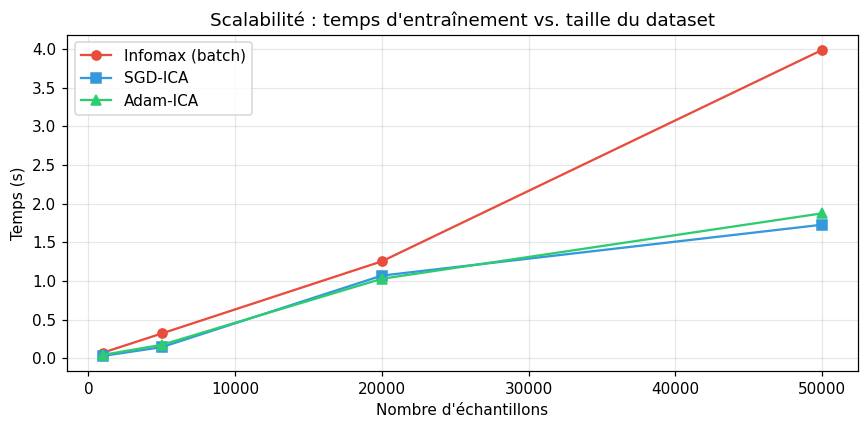
\includegraphics[width=\linewidth]{images/plot5.png}
  \caption{Distribution des composantes latentes $z_j$ pour différentes valeurs de $\beta$.
           À $\beta=0$ (pas de régularisation KL), $z$ suit la distribution native des sources ;
           à $\beta=2$, $z$ converge vers $\mathcal{N}(0,1)$.}
  \label{fig:vae_beta}
\end{figure}

\subsection{Effet de $\lambda_{\text{HSIC}}$ sur l'indépendance}

\begin{figure}[H]
  \centering
  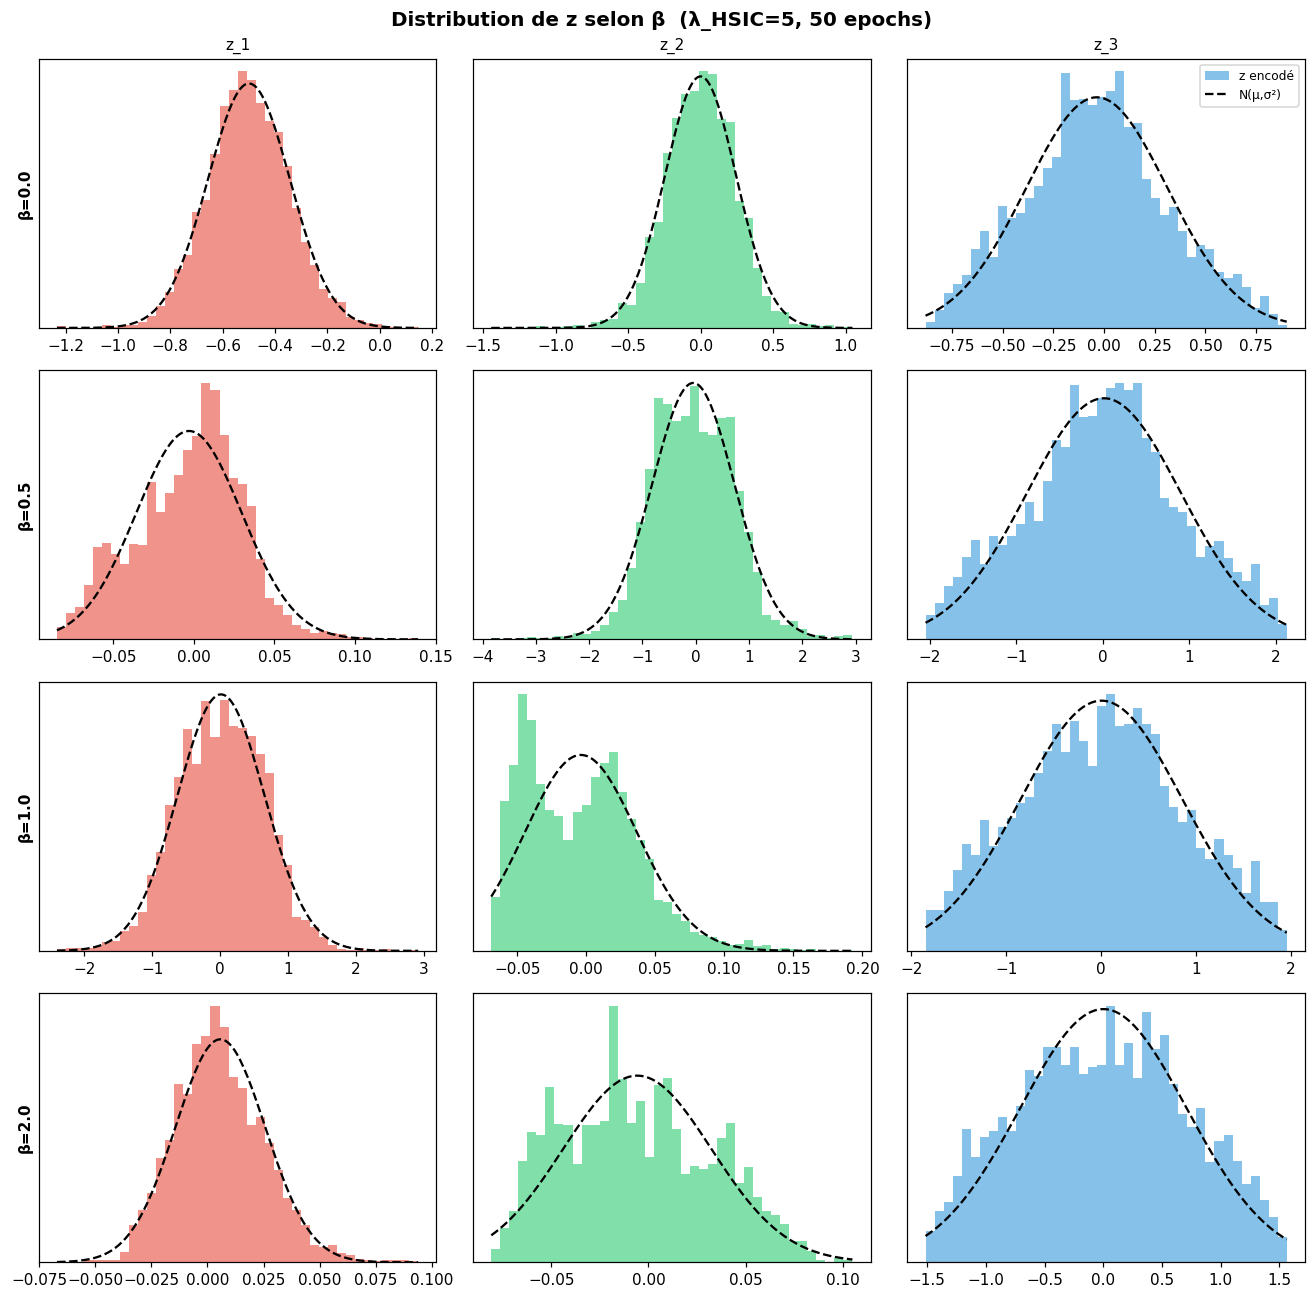
\includegraphics[width=\linewidth]{images/plot6.png}
  \caption{Matrices de corrélation des composantes latentes $z$ pour différentes valeurs
           de $\lambda_{\text{HSIC}}$. Un fort $\lambda$ ($\geq 5$) diagonalise la matrice
           de corrélation, indiquant une indépendance accrue entre les $z_j$.}
  \label{fig:vae_lambda}
\end{figure}

\subsection{Composantes récupérées}

\begin{figure}[H]
  \centering
  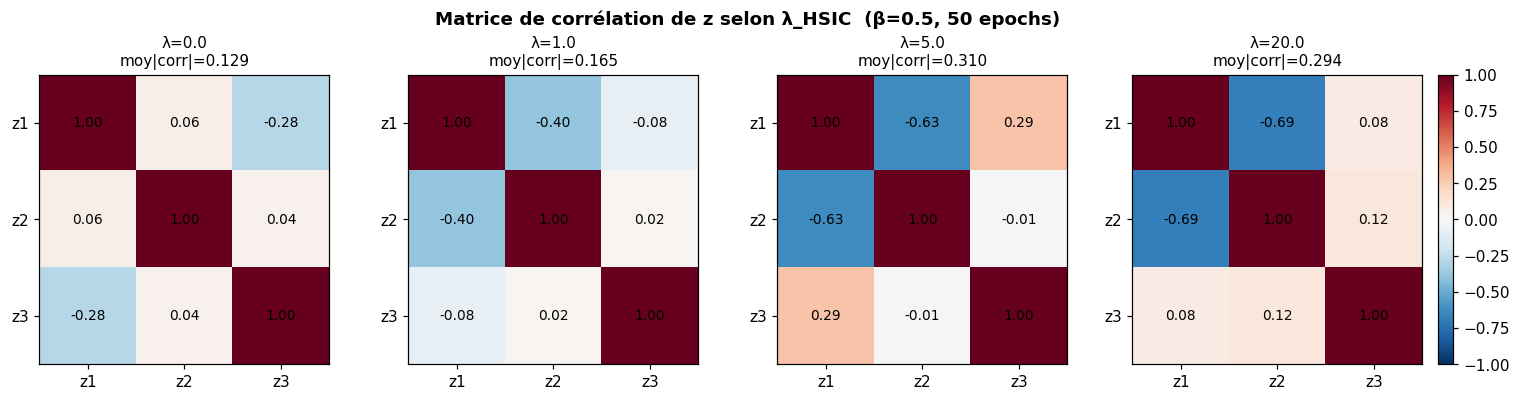
\includegraphics[width=\linewidth]{images/plot7.png}
  \caption{Gauche : courbe de convergence de la perte totale (reconstruction + KL + HSIC).
           Droite : sources vraies (gris) vs composantes VAE-ICA (orange).}
  \label{fig:vae_sources}
\end{figure}

%=============================================================================
\section{Application sur données EEG réelles}
%=============================================================================

\subsection{Contexte}

L'ICA est la technique de référence en neurosciences pour \textbf{séparer les artefacts}
(clignements oculaires EOG, contractions musculaires EMG) des composantes cérébrales dans
les signaux EEG. On utilise le dataset \emph{sample} de MNE-Python \cite{mne2013} :
$f_s = 600\,\text{Hz}$, ${\approx}\,45\,000$ échantillons, $d = 60$ canaux EEG, $k = 20$
composantes extraites.

\subsection{Composantes FastICA}

\begin{figure}[H]
  \centering
  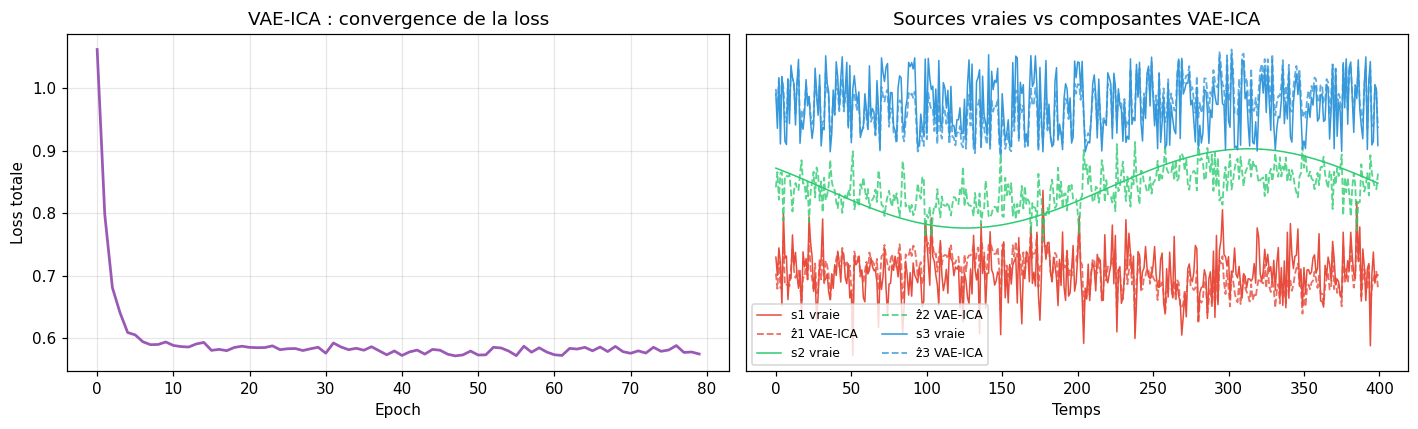
\includegraphics[width=\linewidth]{images/plot8.png}
  \caption{Composantes temporelles extraites par FastICA (sklearn) sur les données EEG.
           Les composantes à forte variance basse fréquence ($< 4\,\text{Hz}$) correspondent
           typiquement aux artefacts oculaires (EOG).}
  \label{fig:eeg_fastica}
\end{figure}

\subsection{Comparaison de l'indépendance}

\begin{figure}[H]
  \centering
  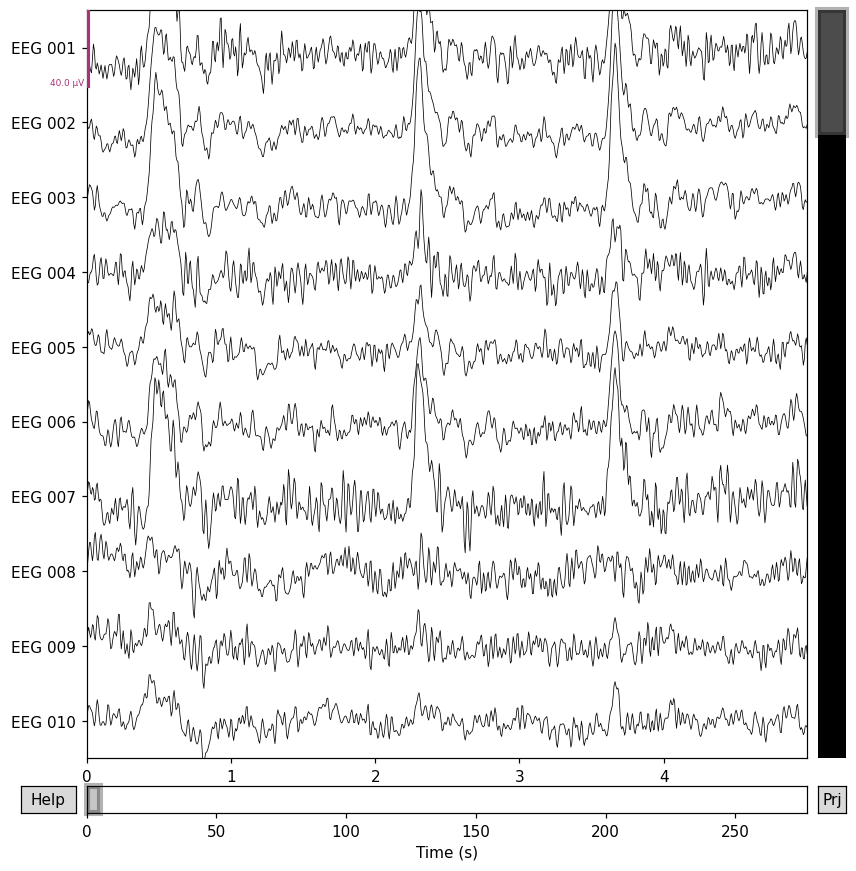
\includegraphics[width=\linewidth]{images/plot9.png}
  \caption{Matrices de corrélation absolue entre composantes : EEG brut (gauche),
           FastICA (centre), VAE-ICA (droite). Un bon ICA produit une matrice
           quasi-diagonale (corrélations hors-diagonale proches de 0).}
  \label{fig:eeg_corr}
\end{figure}

\subsection{Reconstruction après suppression d'artefacts}

\begin{figure}[H]
  \centering
  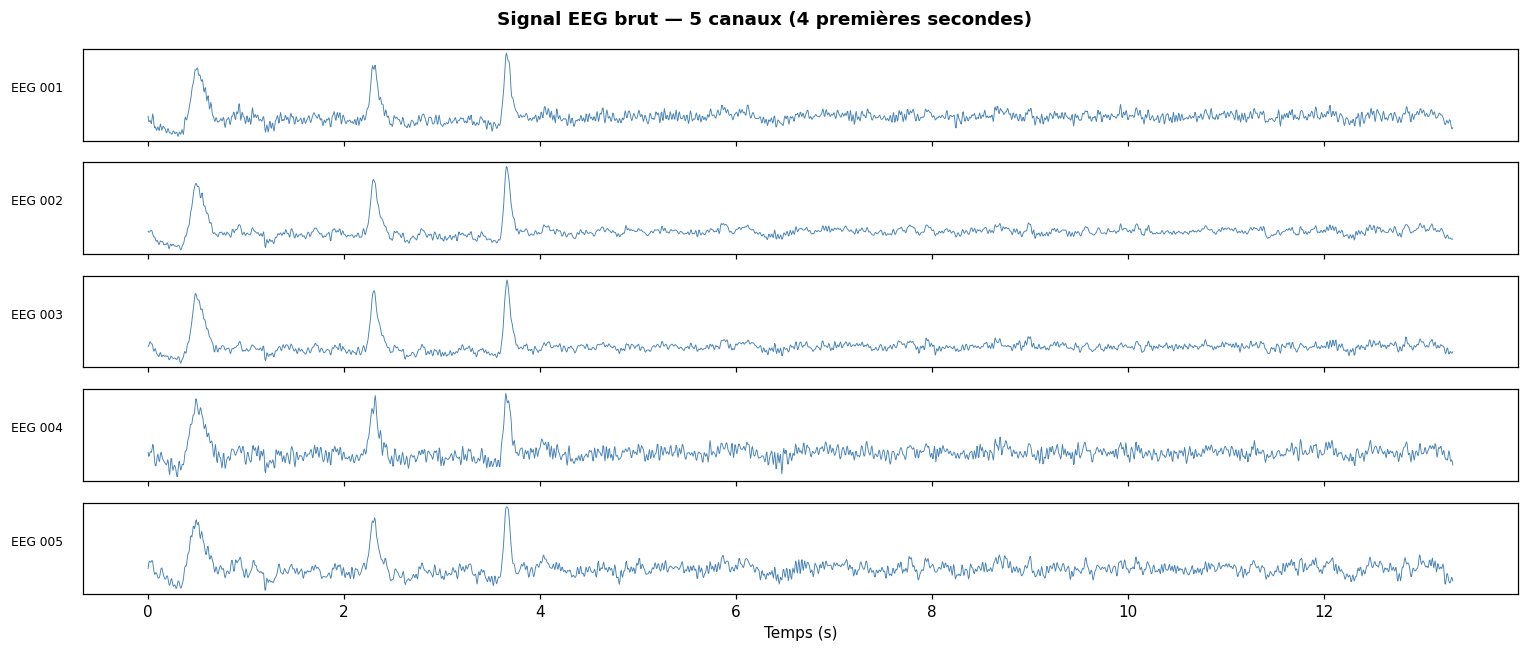
\includegraphics[width=\linewidth]{images/plot10.png}
  \caption{Signal EEG original (haut) et signal reconstruit après suppression des
           composantes artefactuelles identifiées par FastICA (bas). La variance
           basse fréquence est significativement réduite.}
  \label{fig:eeg_reconstruct}
\end{figure}

%=============================================================================
\section{Conclusion}
%=============================================================================

\subsection{Bilan}

\begin{itemize}
  \item \textbf{FastICA} offre la meilleure précision (convergence quadratique) sur des
        données de taille modérée, sans paramètre de pas à régler.
  \item \textbf{Adam-ICA} converge 2--3 fois plus vite que SGD-ICA grâce à l'adaptation
        automatique du pas, tout en restant scalable (mini-batch).
  \item \textbf{VAE-ICA} apprend la distribution des sources sans hypothèse paramétrique,
        au prix d'un coût HSIC en $O(m^2 k^2)$ qui nécessite un sous-échantillonnage pour
        les grands datasets.
  \item Le \textbf{gradient naturel} est la clé commune à Infomax, SGD-ICA et Adam-ICA :
        il rend la mise à jour invariante à la géométrie de $\V$.
\end{itemize}

\subsection{Perspectives}

\begin{itemize}
  \item Online ICA sur flux continus (EEG temps réel, finance haute fréquence).
  \item Sélection automatique de $g$ selon le kurtosis estimé des sources.
  \item VAE-ICA avec prior de mélange de gaussiennes pour sources multimodales.
  \item Extension non-linéaire via normalizing flows.
\end{itemize}

%=============================================================================
%  Références
%=============================================================================
\begin{thebibliography}{9}

\bibitem{bell1995}
Bell, A.~J., \& Sejnowski, T.~J. (1995).
\textit{An information-maximization approach to blind separation and blind deconvolution}.
Neural Computation, \textbf{7}(6), 1129--1159.

\bibitem{hyvarinen1999}
Hyvärinen, A. (1999).
\textit{Fast and robust fixed-point algorithms for independent component analysis}.
IEEE Transactions on Neural Networks, \textbf{10}(3), 626--634.

\bibitem{amari1996}
Amari, S., Cichocki, A., \& Yang, H. (1996).
\textit{A new learning algorithm for blind signal separation}.
Advances in Neural Information Processing Systems (NIPS), 8, 757--763.

\bibitem{kingma2015}
Kingma, D.~P., \& Ba, J. (2015).
\textit{Adam: A method for stochastic optimization}.
International Conference on Learning Representations (ICLR).

\bibitem{gretton2005}
Gretton, A., Bousquet, O., Smola, A., \& Schölkopf, B. (2005).
\textit{Measuring statistical dependence with Hilbert-Schmidt norms}.
Algorithmic Learning Theory (ALT), 63--77.

\bibitem{mne2013}
Gramfort, A. et al. (2013).
\textit{MEG and EEG data analysis with MNE-Python}.
Frontiers in Neuroscience, \textbf{7}, 267.

\end{thebibliography}

\end{document}
